% -*- mode: latex; mode: linkd; mode: auto-fill; mode: flyspell;-*-
\chapter{Design and Implementation}
\label{chap-five}


% Introduction

% Discuss what this chapter will focus on and dive in.
The purpose of this chapter is threefold: it discusses the motivations
that govern the design of the Coglaborate system, such as using the
BioBike chassis~\cite{journals/bioinformatics/MassarTES05} and using
frames as a data structure to represent ACT-R based cognitive models;
it describes the work flow of the system that enables users to build
and share models; finally it discusses in detail a medium-scale model
that was built as a proof of concept, a demonstration of how
Coglaborate would be used in practice.

\section{Problem Definition for Coglaborate}

% This is where I have to discuss what coglaborate is trying to
% achieve 

The primary goal of the Coglaborate system is to provide a
collaborative tool-based environment for the computational cognitive
modeling community. Currently there are no such environments that
provide this facility. Apart from supporting collaboration,
Coglaborate also targets a number of secondary goals:

% Sand boxing 
% Resource sharing
% Tool integration
% Knowledge agglomeration
\begin{itemize}
\item \emph{A sandbox environment}: Currently there are number of
  interesting ACT-R extensions available to modelers. But occasionally
  it might be difficult to set up these extensions.  With a sandbox
  environment, modelers can connect to it and use the module with out
  any setup cost. This has a number of advantages.  The users do not
  have to keep track of the version of the extension and they can
  focus on completing their tasks rather than having to tinker with
  their environment.  Further, developers can work to improve existing
  extensions without as much concern for deployment issues.

\item \emph{Resource Sharing}: When we refer to resource sharing we
  mean sharing hardware. With a Web-based platform that runs on a
  powerful computer, researchers can simulate models that require
  excessive computational power and time.

\item \emph{Tool Integration}: If there are computational tools that a
  model requires they can be hooked in once, as a shared software
  resource.  For example, the R statistical environment can be
  accessed as a library.  Once loaded, the facilities can be accessed
  by many users, who do not need to modify their local environments.

\item \emph{Knowledge Agglomeration}: As modelers explore various
  aspects of cognition, they can contribute their results to a general
  repository that reflects the state of the art.
\end{itemize}

\section{Design Decisions}
% Design Decisions
%       - Why biobike
Two major decisions influenced the design of the project: firstly the
use of the BioBike chassis as a platform to mount the ACT-R framework,
and secondly the use of frames as means to represent ACT-R based
cognitive models in the shared memory. This section discusses the
alternatives that were analyzed and the reasons we made these
decisions.

\subsection{Choice of platform}

% Bio bike and the vision that it is originally based on
We chose the BioBike framework as the platform for the system. This
section examines the basis of that decision by analyzing the
capabilities of BioBike.  BioBike is an instantiation of
KnowOS~\cite{oai:CiteSeerXPSU:10.1.1.75.7132}, a concept based on
knowledge being treated on par with other elements that make up a
computer system.  Operating systems provide useful abstractions for
users to work with the elements of a system.  A simple example is a
file, an abstraction over regions of hardware storage.  An operating
system provide functions by which this file can be renamed, copied,
deleted, and so forth. It also provides further abstractions that
allow significant modifications to raw data. The KnowOS vision extends
this analogy to the realm of knowledge. An implementation of the
KnowOS consists of the following
layers~\cite{oai:CiteSeerXPSU:10.1.1.75.7132}:


\begin{itemize}
\item A knowledge base centered on the frame system.
\item An efficient and extensible programming language that provides
  abstractions for users to work with the system.
\item A Web-based interface to the programming language and to other
  KnowOS services.
\end{itemize}

% Description of biobike
%       - Components
BioBike (originally known as BioLingua) provides biologists with the
ability to perform computational biology operations on large data sets
using a simple language. BioBike ties a number of knowledge bases
together transparently, using a frame-based representation to
represent organisms. As an implementation of the KnowOS vision, it
provides features customized for molecular biologists. These
include~\cite{journals/bioinformatics/MassarTES05}

\begin{itemize}
\item A common framework to access genomic, metabolic and experimental data.
\item A general-purpose programming language (Lisp) customized for
  transparent access to the underlying knowledge bases.
\item A highly interactive environment where code can be evaluated and
  its results displayed immediately.
\item A number of general-purpose tools that help in analyzing interactions.
\item A wiki through which scientists can collaborate and announce results.
\end{itemize}

% Talk about the style of interaction and the result
The BioBike language is built on top of Common Lisp. Users interact
with the system using a Lisp listener. This results in a Unix style of
interaction between the system and the user, where the user types in a
command and can see the results of that action immediately. All Lisp
listeners of the system share the same workspace, which means that
they can also share code.

BioBike provides biologists, in principle, with an environment in
which they interact with the computer in the same terms as they would
interact with their peers; with a uniform framework for accessing
knowledge from a number of different knowledge bases; and with a
common work area where data and results can be shared and external
tools can be integrated.  BioBike has been in place over a number
years and has demonstrated benefits to collaborating teams of
biologists and computer scientists during that time\cite{journals/bioinformatics/MassarTES05}.

\subsubsection{Design Choices}

When making the decision about the platform of the system, another
option we had was to implement a similar system from scratch. But when
we considered the capabilities provided by BioBike (such as a live
Lisp listener, a system for integrating third-party tools, support for
collaboration, and a robust code base) this made the decision of
choosing a platform a trivial one.
%
Further benefits of this decision are related to software engineering
concerns. The code for the system is open sourced under the MIT
license and is actively maintained. As a result we will be able to
download updates to the code and apply those changes in a way we see
fit to the system.

\subsection{Choice of structure for representation}
% Introduction
A structured representation of an ACT-R model is intended to provide
an abstraction above the level of modeling code An abstraction should
give a number of benefits: the ability to share models more
conveniently than by exchanging Lisp code; the potential for an
``ecosystem'' of tools for to support ACT-R modeling, in construction
and analysis; and the ability to maintain revisions of
models\footnote{This is a continuing concern in ACT-R modeling
  research.  The ACT-R architecture has gone through several major
  revisions over the years (the current version is ACT-R 6.0, but
  modeling researchers rarely return to models based on earlier
  versions to test whether changes in the implicit architectural
  dependencies have rendered their past work invalid.  Improved
  modeling abstractions may make this process easier.}
%
and the ability to extend ACT-R models in ways explicitly planned for.

We had to decide between three main choices of structures for
representing an ACT-R model: a direct representation of models in the
ACT-R modeling language, a semantic network, and frames.

%       - Direct representation: that is store the entire code as some variable
ACT-R models are essentially Lisp data structures. Therefore the
direct representation of the model would store the code for the model
as is. The benefit of this approach lies in the simplicity of the
implementation, which would have involved storing the code as symbols,
and the ease with which modeling researchers can understand a familiar
representation. But this approach has a number of disadvantages.
Building tools for this representation would be exceptionally hard
because the tools would have to parse the model before being able to
perform any operations.  The representation does not allow us to store
meta data.  It does not allow us to easily add capabilities for reuse
of the model.  Finally it would be cumbersome to implement a system of
revision control for this data structure.

%       - Semantic Nets
%         - Describe Semantic nets
An alternative to the direct representation is using semantic networks
to represent ACT-R models. Semantic networks are a notation for
representing knowledge, using nodes to represent objects, concepts or
situations in a domain, and using arcs to represent relations between
them~\cite{Sowa87,Barr81}. This would mean representing the internal
components of ACT-R models as node: the productions, and the
conditions and actions they contain, as well as models themselves.
The advantages of using this representation are that tools written for
ACT-R could act directly on the nodes representing productions and
models; the representation would make it easy to implement facilities
for reuse of productions; queries could be constructed to determine
the type of objects and their relationships. The deficiencies of this
representation are that implementing a system of revision control
would be difficult because we would not be able to represent version
information in a straightforward way.  It would also be difficult to
add capabilities of model reuse.

%       - Why frames
% -     Describe frames
% Brief description of other possible structures if I had not used
% frames.

The frame data structure was introduced by Marvin
Minsky~\cite{Minsky1974a} in 1975, in one the seminal papers in the
area of knowledge representation. Frames are structures that can
represent objects, situations and concepts. Frames are arranged in a
hierarchical taxonomy where every frame is linked with its parent
frame. The parent frame represents a more general concept than its
child\cite{karp-93}. A frame is made up of a number of slots. Slots
define the properties of the object being represented by the
frame. Slots are sometimes also used to represent relationships
between two frames. This representation provides us with a number of
advantages.  Unlike semantic networks we have all related data stored
in a single frame; frames are dynamic and allow slots and their values
to be updated very easily.  Since frames are structured, it is easy to
write tools to help perform various forms of analysis.  Finally, in
the future frames might help in analyzing more complex forms of reuse
of cognitive models.

In knowledge representation research it is common to find integrations
of frames and semantic networks; for example, a semantic network might
include frames rather than atomic symbolic concepts in its nodes.  The
distinctions made in the above discussion are between their ``core''
properties.

% Describe frames in reasonable amount of detail.

% describe why are frames the sweetest things since sliced bread...

\section{System Design}

\begin{figure}[htp]
  \centering
  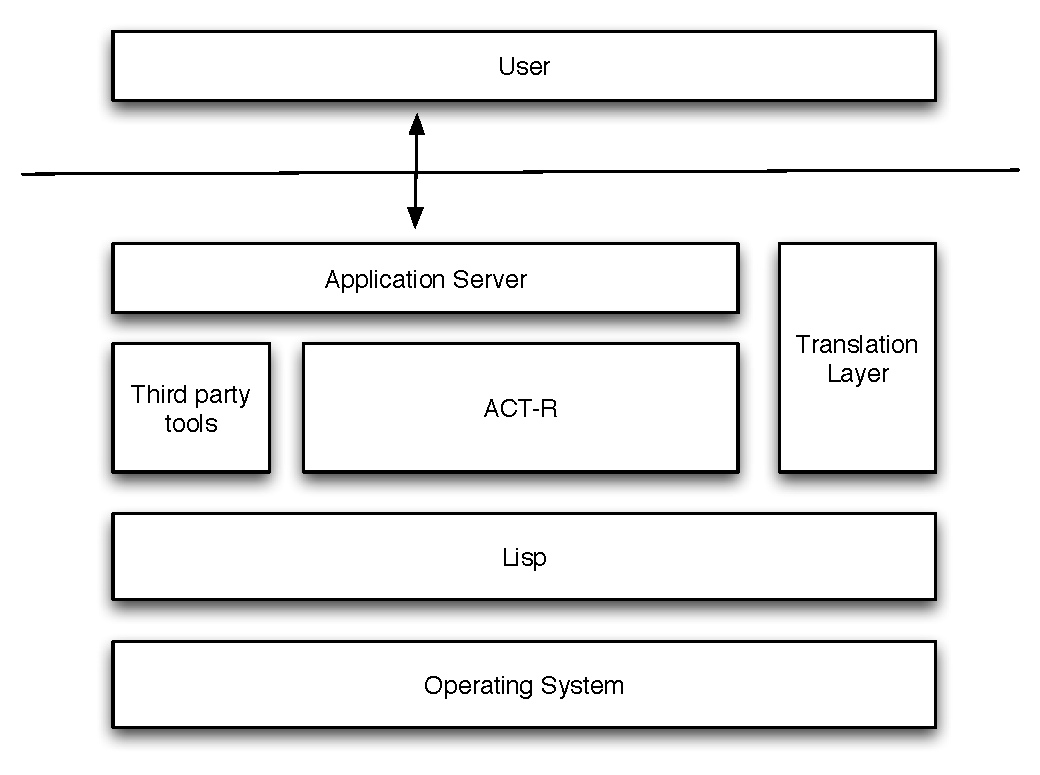
\includegraphics[width=90mm]{SystemOverview}
  \caption{System Design}
  \label{SysOverview}
\end{figure}

This section aims to explain how various components of the system work
together to have the desired effect. Figure \ref{SysOverview} provides
a high level overview of the system.  This section will examine each
component in detail.  The system currently runs on a server running
GNU\slash Linux.  As a result we have a secure, robust, and stable
platform on which to base our system.

%\subsubsection{Operating System}
% there obviously is no need to introduce the operating system. 
% The system currently runs on a GNU/Linux based machine. 

\subsubsection{The User}

The user interacts with the system through a web browser. When a user
logs in he is put into the ACT-R package. This is done because it was
not possible to export all the required variables and functions into
the user package. This is because ACT-R either lets us export all its
symbols into to the \texttt{cl-user} package or the \texttt{act-r}
package. 

The only thing different about the models being written to run on
their own system and those that are run on the Coglaborate system is
that the users have to wrap their code with a call to the
\texttt{with-user-meta-process} macro. This macro creates new meta
process for the user and lets them run the model in that ACT-R meta
process so as to avoid conflicts with other users running their models
in ACT-R. 

\subsubsection{Application Server}

% Describe the application server. Dont know if I have to describe the
% flow of code
We use the AllegroServe Web Application server to serve the front end
that the user sees. The AllegroServe\cite{aserve2009} application server provides us
with: a HTTP/1.1 compliant web server capable of serving static and
dynamic pages; a HTML generation facility that allows us to merge
static and dynamic content; secure socket layer for the server and
clients; a comprehensive test suite to verify the functionality of the
client, server, proxy and SSL. It is licensed under the Lisp Lesser
GNU Public License. 

%\subsubsection{Lisp}

% Do I advocate the use of lisp here or do I just describe the version
% being used and its benefits

\subsubsection{ACT-R}

When a user evaluates a model it is compiled by the ACT-R model into a
thunk. My code is plugged into the parser of the ACT-R compiler so
that we can access the data structure that is generated as the model
is parsed. This data structure is then converted into frames. A
detailed description of the structure of the frames can be found in
the following sections.




\subsubsection{Translation Layer}

This is a conceptual layer that represents the implementation of the
ideas suggested in this project. This layer consists of two main
sections: a section that converts ACT-R model data structures into
frames and a section that converts frames back into ACT-R
models. Since the code in this section is trivial, this section aims
to explain the structure of the frames that are created. Every frame
has a few elements in common that describe: the type of object that the
current frame represents and the name of the object that the frame
represents. The structure of all the frames created by the code is
described below.

%TODO: Put in a diagram that shows these frames in a hierarchical fashion

\begin{itemize}
\item \emph{The model frame:} A model frame represents an ACT-R
  model. It consists of a code slot that holds all the code that is
  required by the model: this includes code for initialization of the
  model and miscellaneous utility functions that may be required by
  the model. It has a slot for productions that are a part of the
  model.
\item \emph{The production frame:} A production frame consists of a
  conditions slot, which defines the conditions that are required for
  the condition to fire, and a actions slot which lists all the
  actions that will be executed if that production is fired.
\item \emph{The buffer test frames:} Every production in ACT-R consists
  of a number of conditions. Each condition consists of a number of
  tests. Each buffer test frame represents one such test. This frame
  has a slot to represent individual clauses within the test.
\item \emph{The conditions frames:} The conditions frames represent an
  individual clause it consists of a test field that represents the
  buffer variable it is testing and a value field that represents a
  value against which we are testing it. This field can also hold
  variable as in ACT-R productions.
\item \emph{The buffer actions frames:} ACT-R productions can perform
  a number of actions that can either modify, clear or retrieve a
  chunk in a buffer. These actions are represented by these frames.
\item \emph{The action frames:} Individual clauses that represent the
  modifications that are required to be made to the buffer are
  represented by these frames.
\end{itemize}

The names of the all frames except the name of the frame that represents
the model are appended with a random symbol so as to avoid name
clashes. 

%Describe what happens here....draw diagrams to show frames from
%various levels...for example frames that represent productions,
%models, actions and conditions.

When a user clicks a link representing the frame a function named
html-for-browse-frame is called. This function searches for the frame
and then converts it to code which is then returned to the browser.


\section{Work Flow}

This section illustrates a scenario where a user creates a model and
evaluates it. Another user comes in searches for the model created by
the first user, navigates around its productions and obtains the code for
it. 

\begin{figure}[htp]
  \centering
  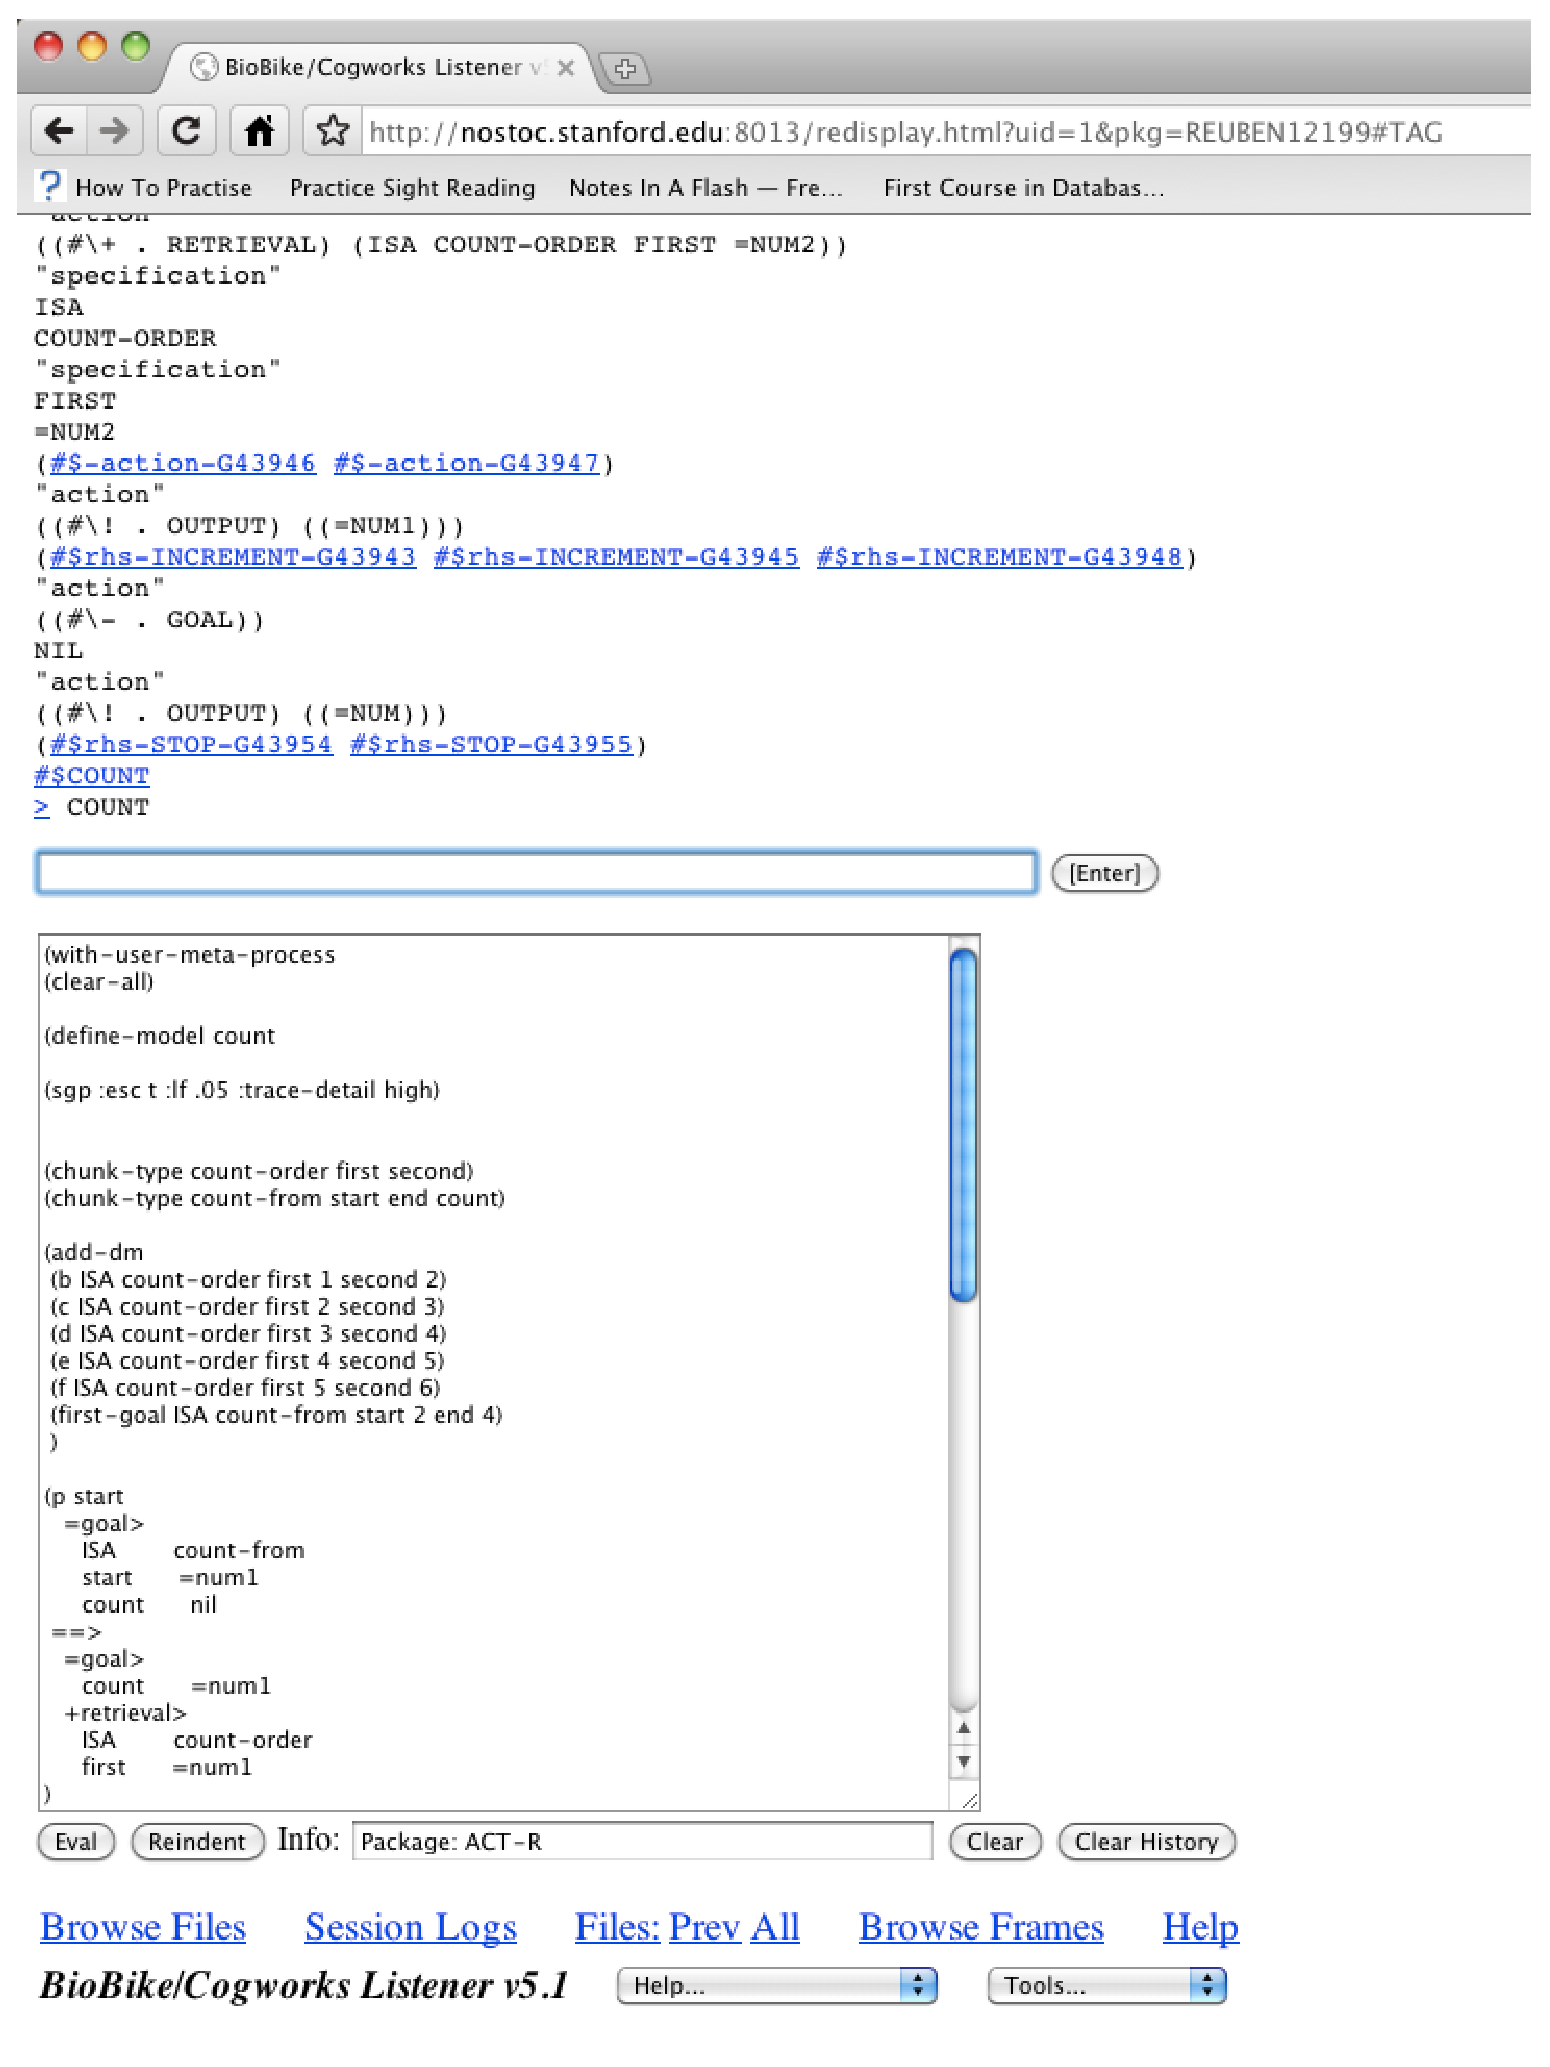
\includegraphics[width=90mm]{UserCreatesModel}
  \caption{A user creates and evaluates a model}
  \label{UserCreatesModel}
\end{figure}

A user creates a frame representation by evaluating the code that he
types into his lisp listener as shown in figure
\ref{UserCreatesModel}. The lisp listener has two text boxes, the
large text area is used to type in complete models and the smaller
text box is used to type in one off commands.

\begin{figure}[htp]
  \centering
  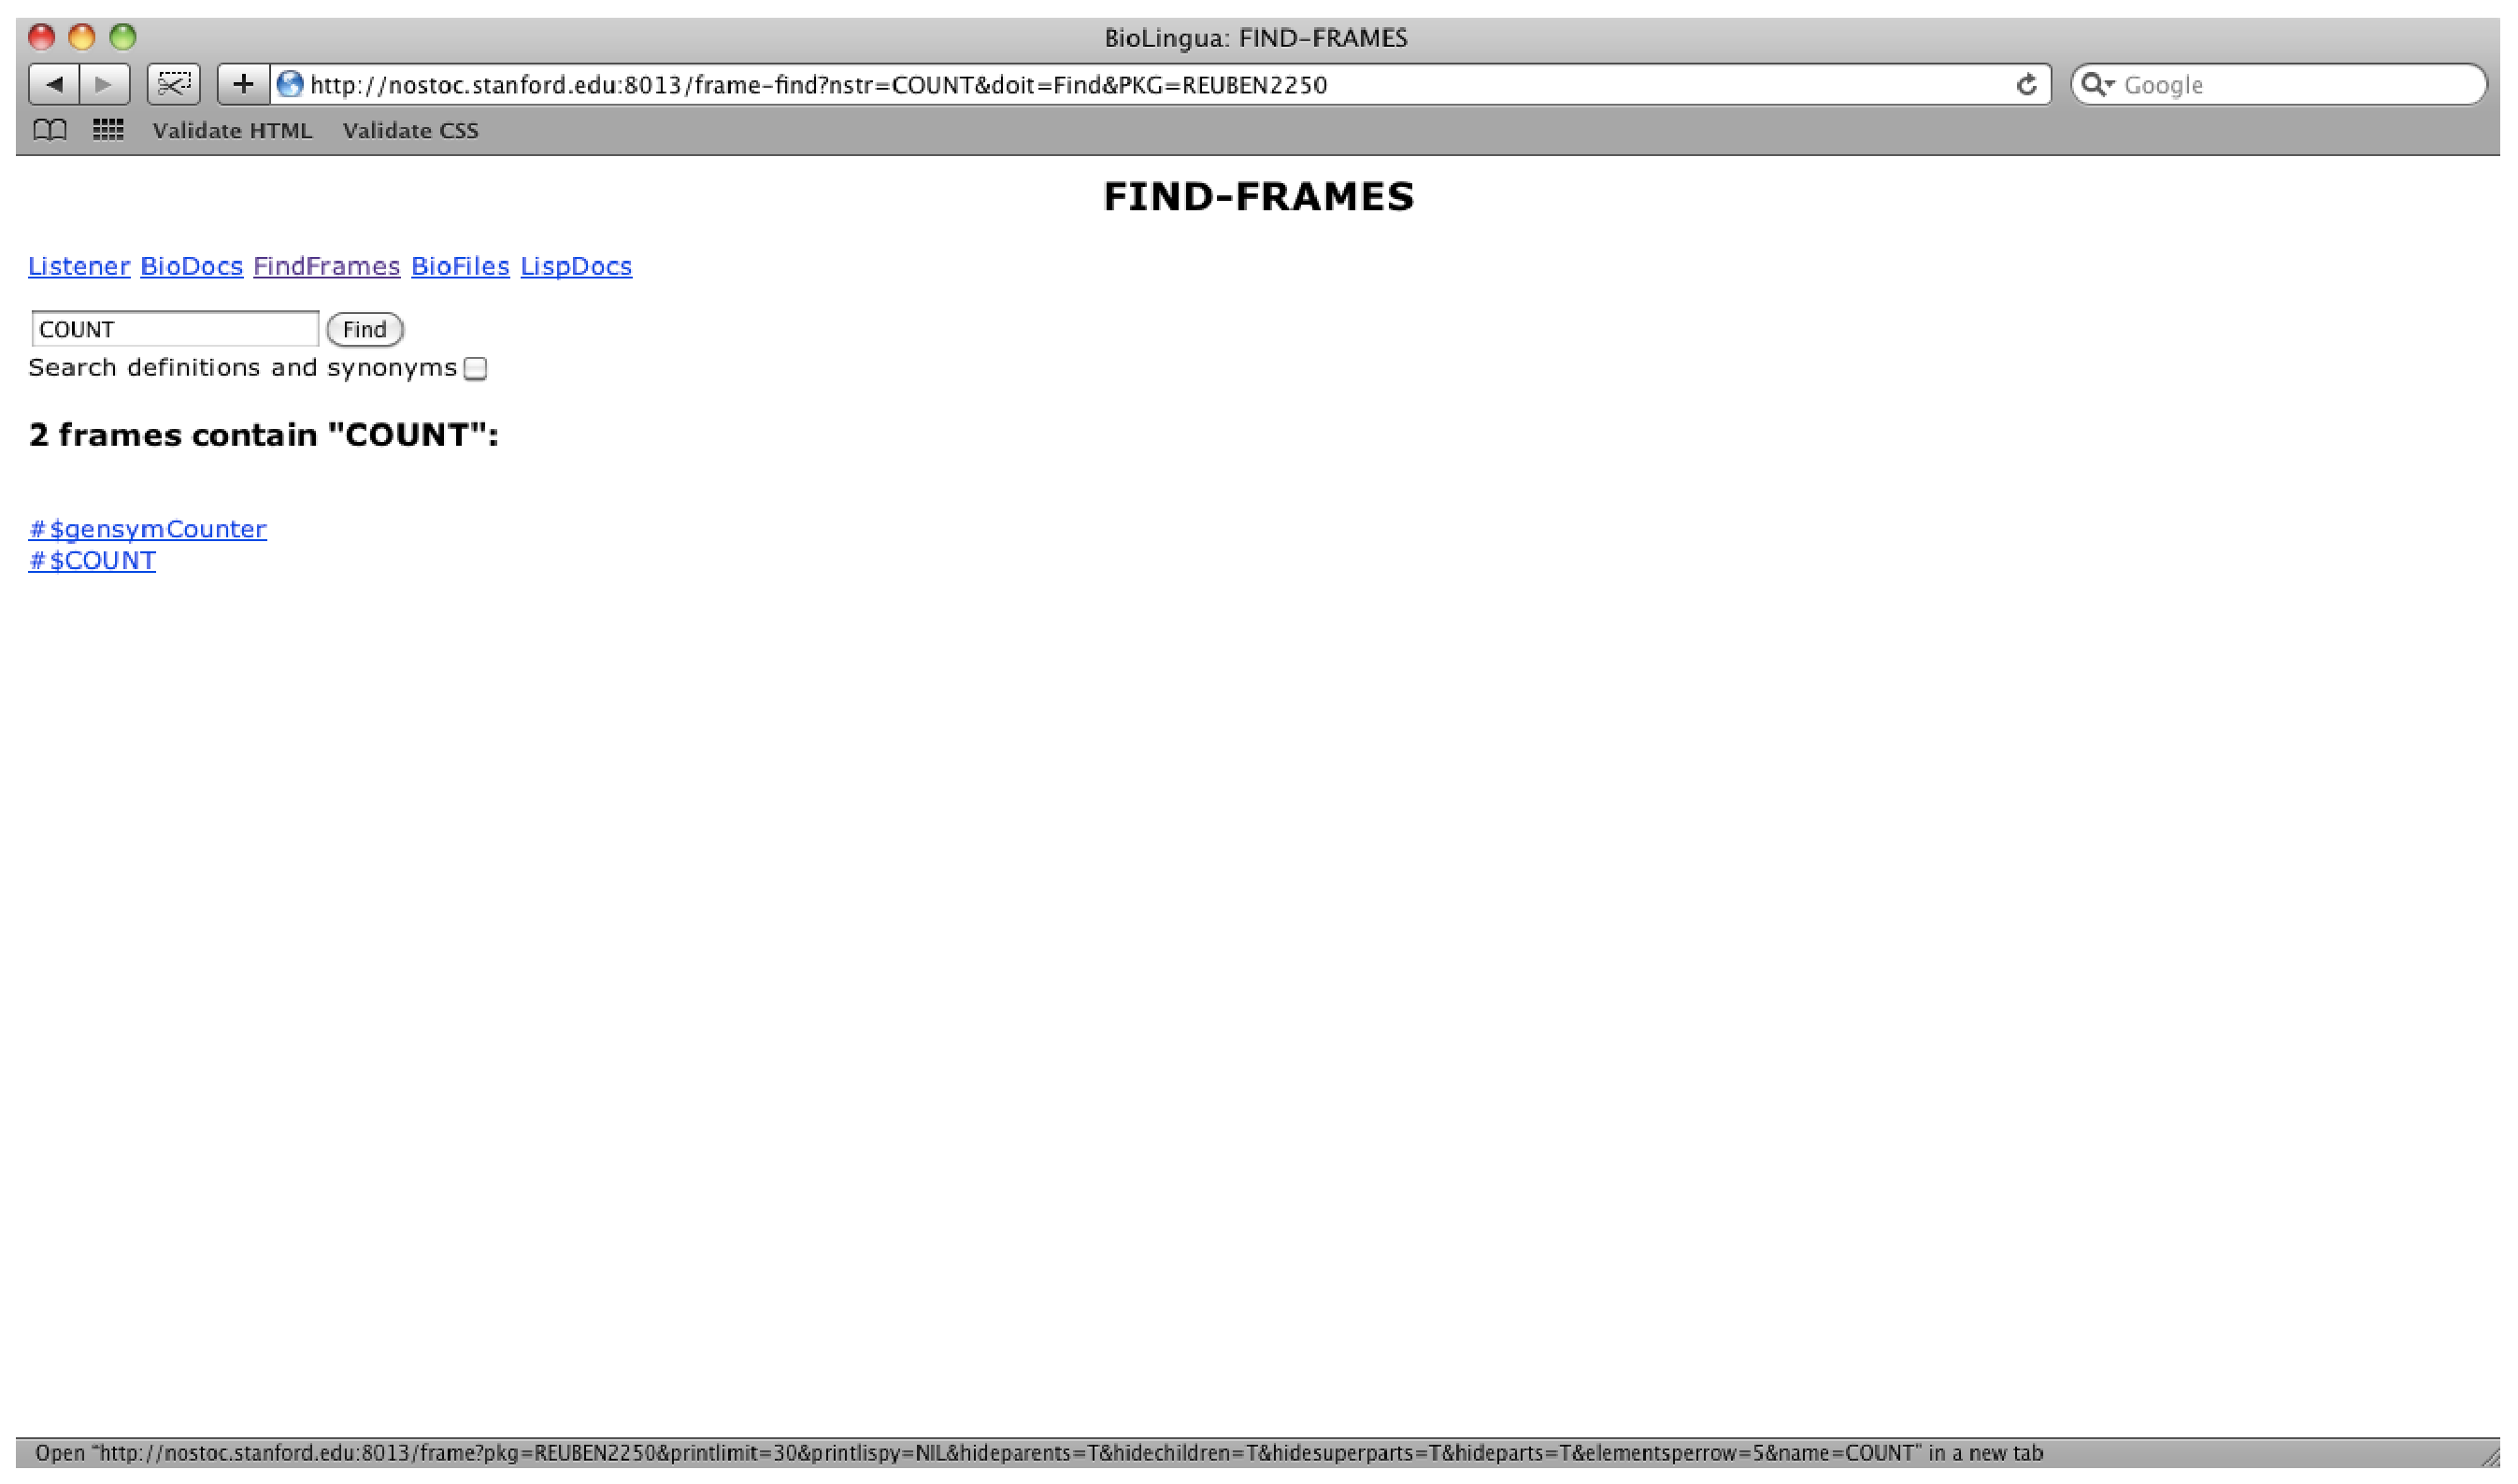
\includegraphics[width=100mm]{SearchForModel}
  \caption{Search results after searching for a model}
  \label{SearchForModel}
\end{figure}

Once a frame representation of the model has been created any other
user can search for the model if he knows the name of the model. This
is done by clicking the ``Find Frames'' link. The result of the search
is shown in figure \ref{SearchForModel}.

\begin{figure}[htp]
  \centering
  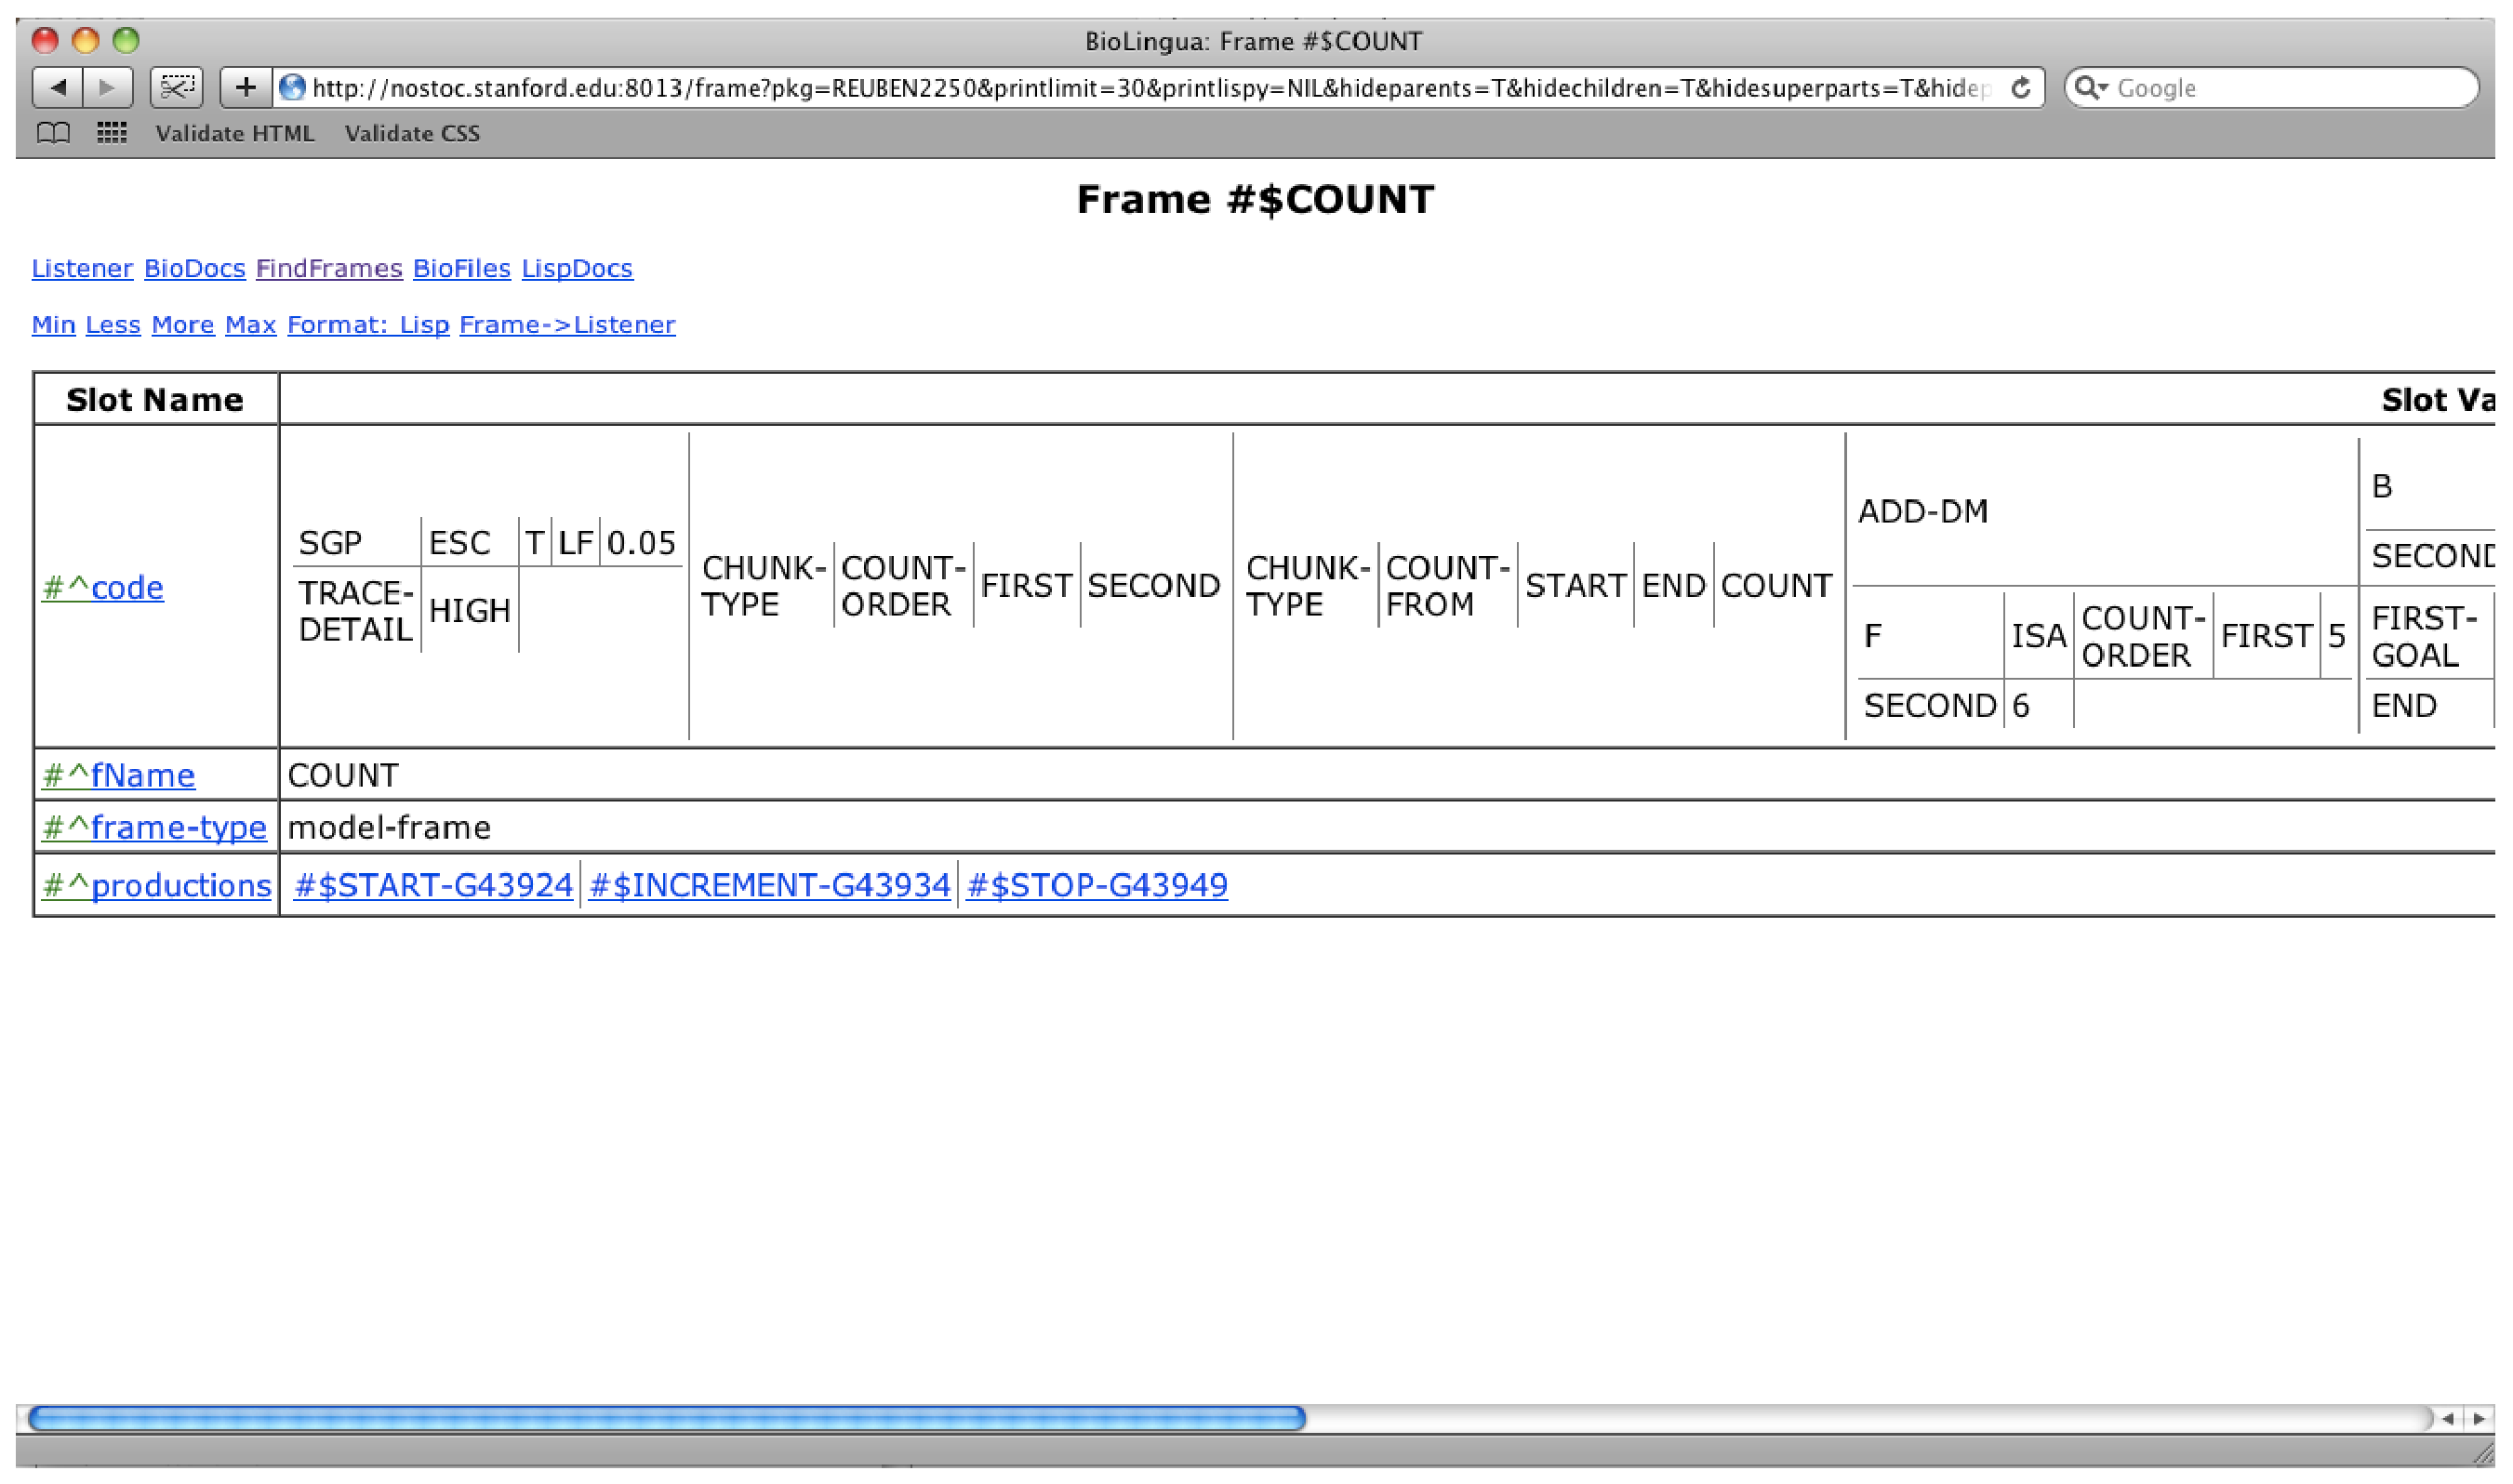
\includegraphics[width=100mm]{NavigateFrame}
  \caption{Navigating a model represented as a frame}
  \label{NavigateFrame}
\end{figure}

Figure \ref{NavigateFrame} shows the frame representation of what the
model that the user was searching for. Once the user finds the model
that he was searching for, he can navigate the model by clicking on
the links inside the frame table.

\begin{figure}[htp]
  \centering
  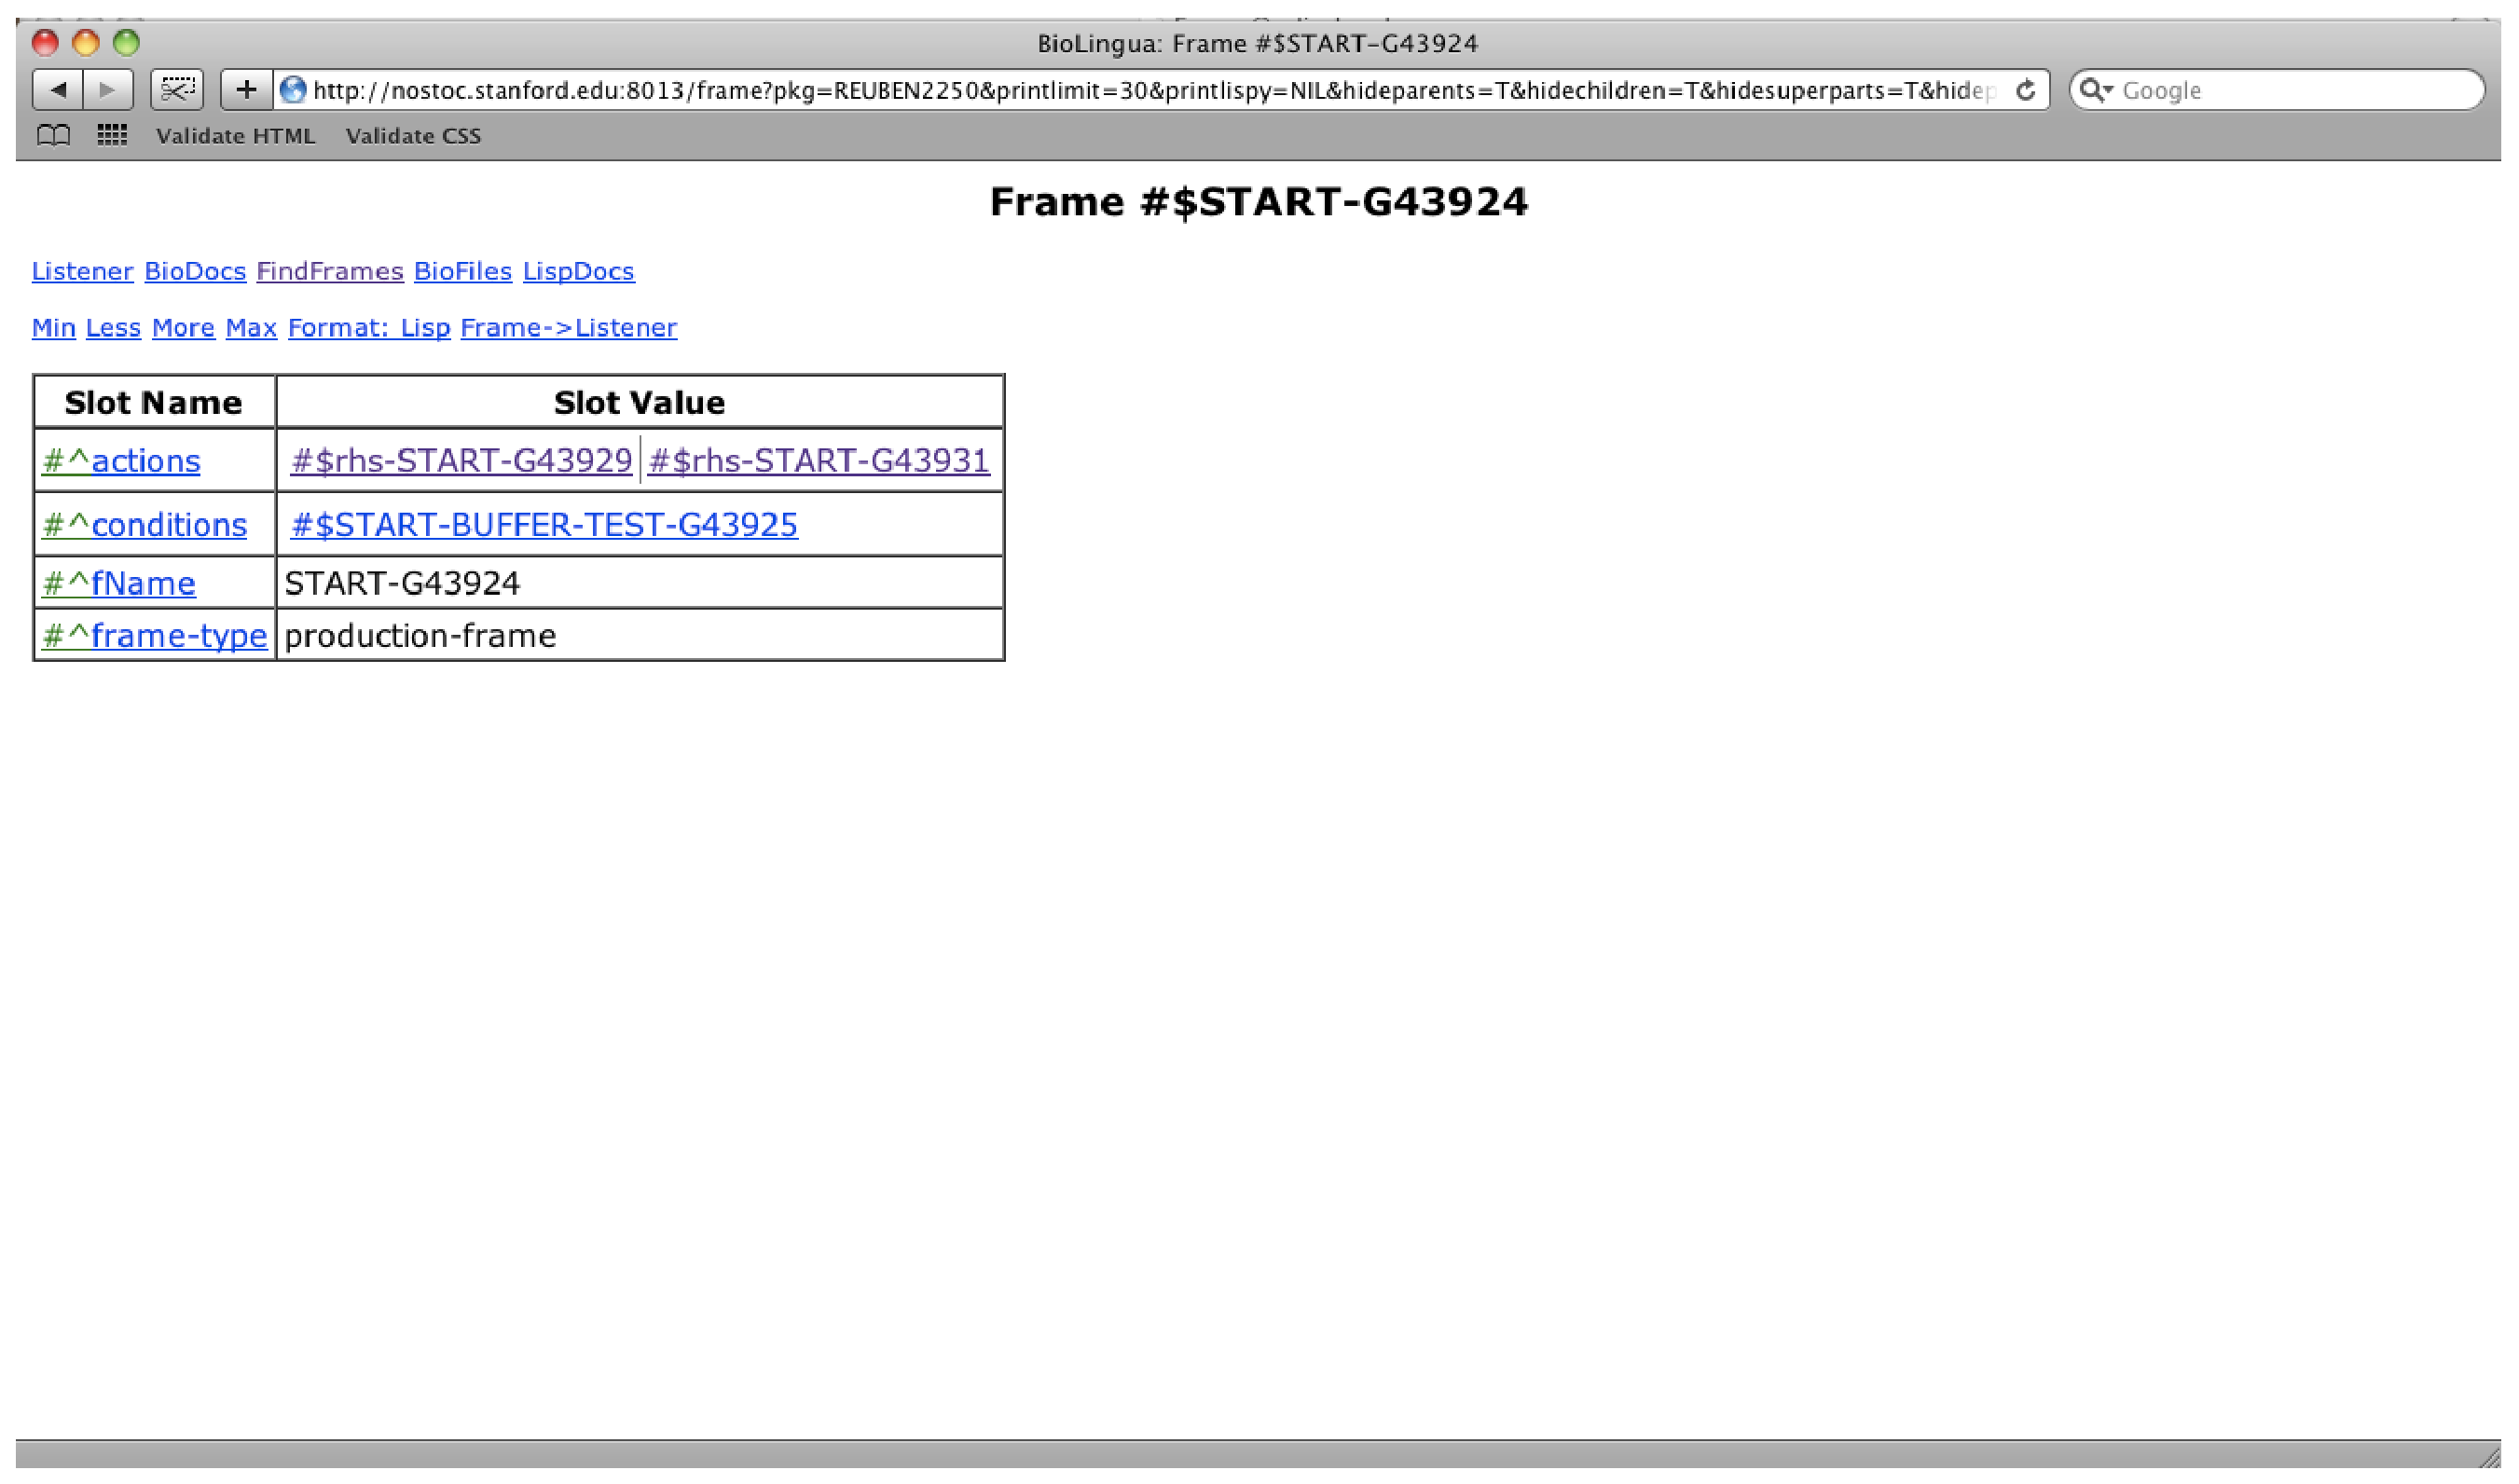
\includegraphics[width=100mm]{NavigatingAProduction}
  \caption{Navigating a production represented as a frame}
  \label{NavigatingAProduction}
\end{figure}

Figure \ref{NavigatingAProduction} shows us the frame representation
of a production, this is obtained by clicking any link in the slot
value column of the model frame for the slot name ``productions''. The
user can investigate a production further by clicking on the links in
the slot value section. 

\begin{figure}[htp]
  \centering
  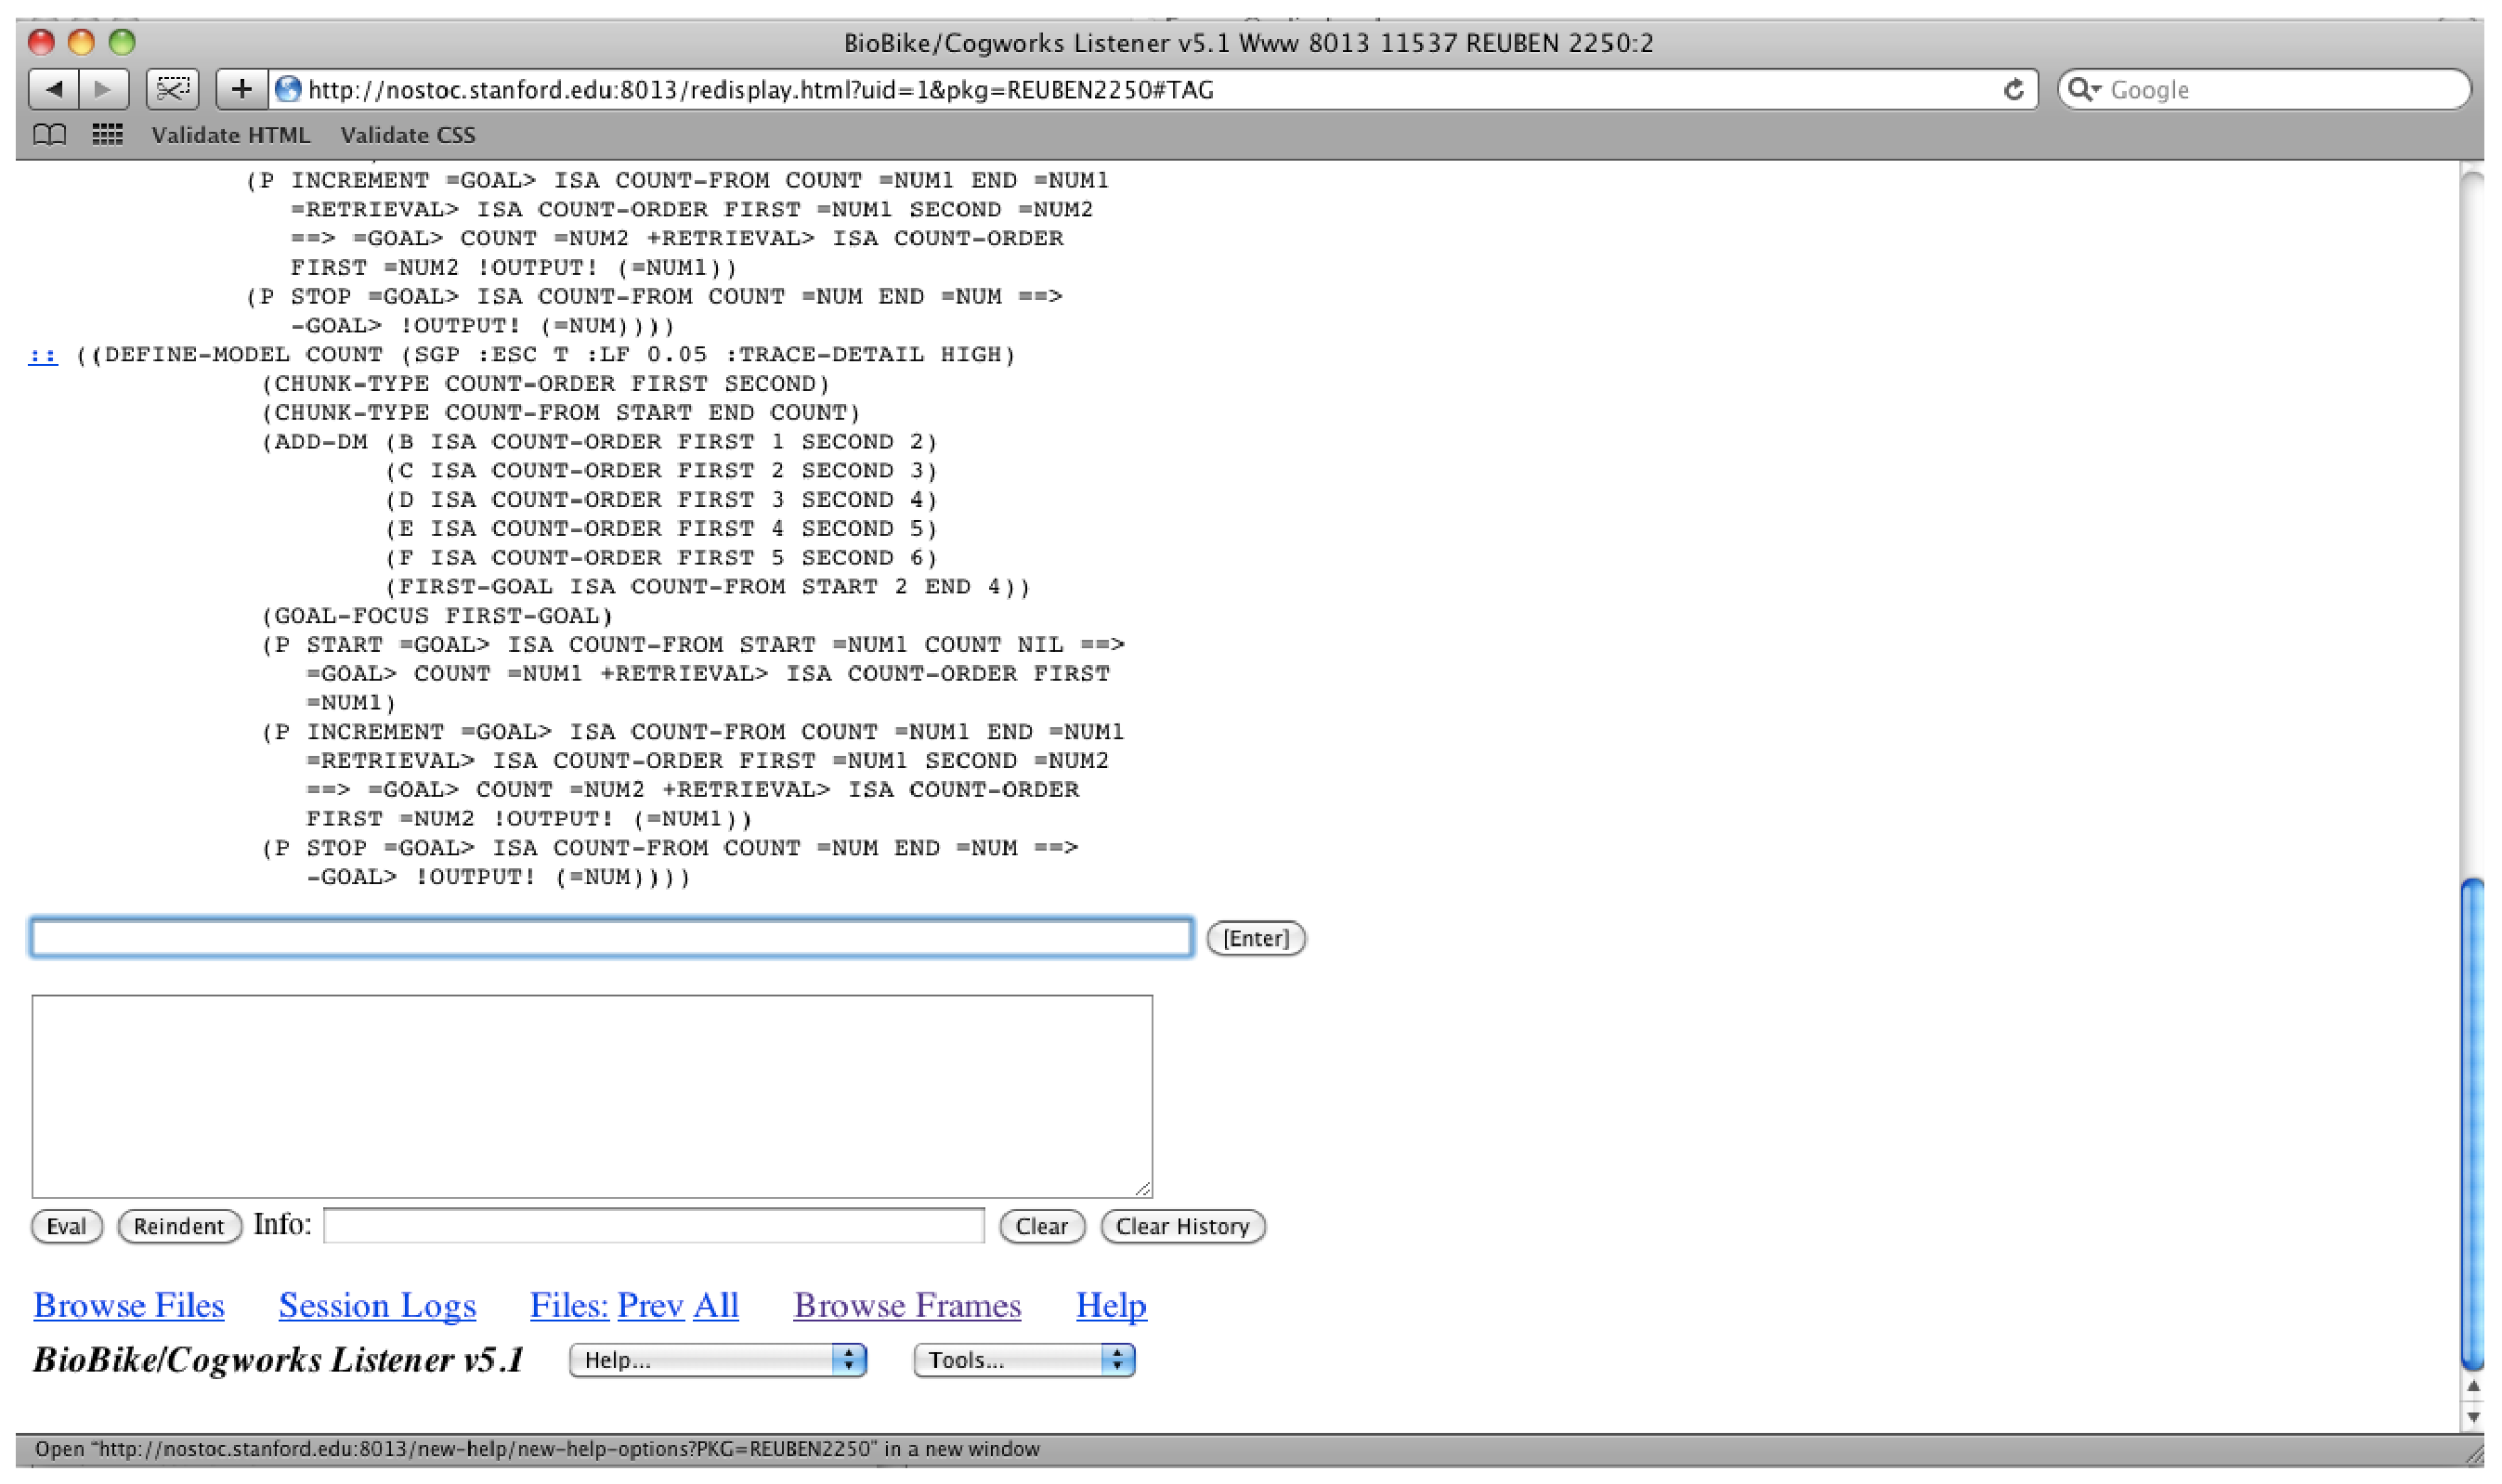
\includegraphics[width=100mm]{ConvertFrameToImage}
  \caption{The resultant code after clicking the Frame $\rightarrow$ Listener
    link}
  \label{ConvertFrameToImage}
\end{figure}

If a user wants to obtain code for the model he can click the
Frame$\rightarrow$Listener link on the index page of the model. Figure
\ref{ConvertFrameToImage} shows the resulting code generated as a
result of clicking the said link.

% Coglaborate
%       - Describe work flow that shows collaboration occurs with screen shots.
%       - Describe what was modified and why
%         - Describe how frames are created
%         - Describe how the reverse procedure is implemented

\section{Proof of concept}

% Proof of concept
%        - Problem description
%        - Approaches
%        - Approach taken
%        - What can be deduced from it.

% Explain the need 
% What are we trying to prove by this proof of concept

% 1) The system can handle medium sized models

% 2) It provides us with the benefits we set out when we set out to
% develop this project

To evaluate the capabilities of the system we built a simple but a
medium scale models. The essence of this exercise are two fold:
firstly we show that the system is capable of performing a non-trivial
cognitive modeling exercise and secondly to demonstrate the level of
maturity of the system. This section discusses the problem description,
the approaches that we have chosen and what we can deduce from this.

\subsection{Problem description}

% Give a brief description of the problem
%Describe the crossword
%describe synonyms
A crossword puzzle is a puzzle in which words or phrases are entered
into an interlocking grid either horizontally or vertically. The words
are determined by a series of clues that define the word or the
phrase. Two or more words are synonyms if they can be exchanged in the
same context while maintaining the meaning of the context. Our proof
of concept problem is a crossword puzzle where the clues and the
solutions are defined as being synonyms of each other.


%Describe why is this a good idea
This problem is an appropriate problem to choose for the following
reasons: it demonstrates that this system is a practical system and is
ready for the outside world, albeit the code needs little bit of
polishing; it demonstrates that users can use this system to write and
test sand boxed act-r modules and finally it places considerable
demands on the hardware of the computer, in terms of memory and
CPU. As a consequence we can demonstrate that we have achieved most of
the objectives we had in mind for the system.

\subsection{Implementation}

% Start up by describing wordnet
The data that helps us determine the solution to our clues is provided
by WordNet\cite{journals/cacm/Miller95}. Miller defines WordNet in the
following terms:

\begin{quote}
  WordNet is an online lexical database designed for use under
  program control. English nouns, verbs, adjectives, and adverbs are
  organized into sets of synonyms, each representing a lexicalized
  concept. Semantic relations link the synonym sets. 
\end{quote}

% Describe the WordNet module
We use a module(WNLexical) that enables ACT-R to make use of the
WordNet lexical database. The module does so by converting the WordNet
database into set of s-expressions that can be read in by the
WNLexical module and stored as ACT-R chunks. The WNLexical module
exposes its functionality through the means of an ACT-R buffer, aptly
named \texttt{wn-lexical}. This buffer can query the WordNet database
for synonyms, antonyms, hyponyms, meronyms, glossaries of words
etc. The results of these queries are available from accessing the
slots of the buffer.


% Describe the data strcutre module,
%%% Discuss its capabilitis
%%% Dicusss the interfaces it exposes
% Explain how constraints are be maintained.
%TODO: Draw a diagram that shows an abstract representation of the
%crossword puzzle.
The data structure for the clues is exceedingly simple. The data
structure is a list of clues(which are represented as chunks), where
every clue is a list that consists of the starting co-ordinates of the
word, the direction(either across or down), the clue string, a
location to put in a solution and the actual solution itself. The data
structure is manipulated using a the \texttt{Crossword} module. The
crossword module has the ability: to set words in the specified
location; to verify if the crossword still maintains constraints and
to query various parameters of a specific clue.

% Describe the productions
% Describe the algorithm
When the model(the source code of the model is available in appendix
A) is evaluated it initializes three chunk definitions: a chunk type
to maintain the state of the goal buffer initially; a chunk type that
defines the clue and a chunk type that maintains the state of the goal
buffer as we actually get into the process of solving the
crossword. It sets up a few parameters so as to prevent the decay of
crossword chunks in the memory. We then check the memory to see if we
can find any clues that have not been added to the data structure. If
we find a chunk that has not been added to the crossword we add it
in. Once added in we update the goal to find all the synsets of the
word. This is done by querying the WordNet module. For every synset
found we create a chunk using the \texttt{imaginal} module. If we
cannot find the word we display an error message. For every chunk that
we had created earlier, we query WordNet to obtain all the words
in the synset if the word we have found matches the solution we set it
in the clue and mark the clue as solved. This process repeats till all
the clues have been solved or have been marked as being unsolvable.

%TODO: do I put in a high level view of the algorithm?
The output trace of this model is available in Appendix B. It shows
the trace for two words: one where we are able to solve the clue the
other being unsolvable. The trace clearly shows the working of the
algorithm in explicit detail.

\subsection{Conclusions}

% Talk about why the system is usable
The proof of concept demonstrates that we have a system that can be
used in the real world. We can assert this claim with confidence
because we have been able to write and run a medium scale model on the
system. 

% Show that the objectives that we set out to meet have been met.
We can further assert that we have met most of the objectives that we
had set for ourselves through this model: we set up an environment
where any other researcher can work with the WordNet module, we also
wrote up a module that was required for the data structure; we can
demonstrate the capability of resource sharing, running the model on
my personal computer brought my computer down to a crawl because the
WordNet module loads all the chunks into memory, whereas the model ran
fine when run off the server and although the model did not make use
of any third party tools, the system has a regular expression library
and a package management, Another System Definition Facility(ASDF), 
system integrated into it.

% Effort.
The project added about 1000 lines of code to the existing code
base. That figure does not include the lines of code of the model. The
challenges faced during the development of the project involved:
deciding the structure of the frames so that we have a right level of
granularity and at the same time we don't loose any information
related to the productions; designing a way so that using the system
is as intuitive to the user as can be; figuring out a way to provide
collaboration using frames; analyzing the ACT-R compiler to identify
locations where the translation layer would hook in and, identifying
and fixing a couple of existing bugs in the existing system.

An evaluation of the collaborative aspects of the use of Coglaborate
are unfortunately beyond the scope of this thesis.  Some evidence for
this capability is provided by experience with BioBike; some
similarities in the benefits can be expected.  Nevertheless an
illustration of the use of Coglaborate to solve a medium-sized problem
should gives us insight into some of the strengths and weaknesses of
the approach.







